\chapter{What? Main paradigms regarding the nature of Dark Matter}\label{paradigms}

\begin{figure}[t]
$$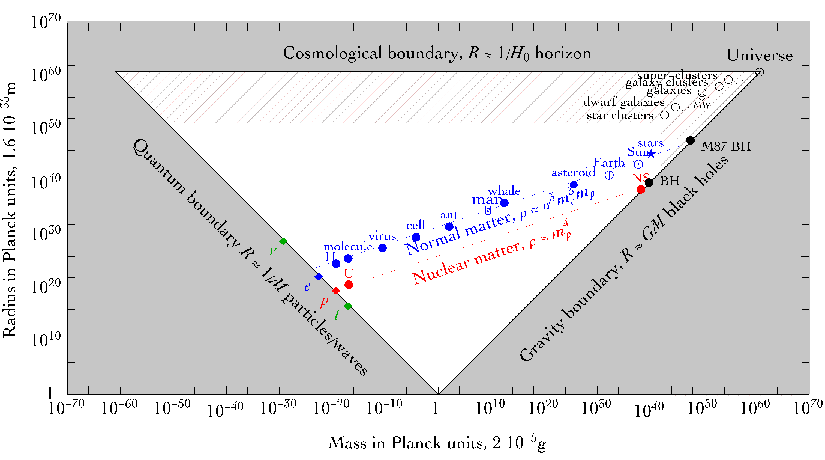
\includegraphics[width=0.85\textwidth]{figs/MassRadiusCatalogue}$$
\caption[Catalogue of the Universe]{\em\label{fig:catalogue} {\bfseries Catalogue of the Universe} in the plane $($mass, radius$) = (M,R)$.
Normal matter forms objects around the blue dashed line, i.e.~with density $\rho\sim M/R^3 \sim \alpha^3m_p m_e^3$.
Nuclear matter forms objects around the red dot-dashed line, with density $\rho\sim m_p^4$, going from hadrons and nuclei to neutron stars, close to the black hole limit.
DM is believed to be relevant for understanding the largest structures of the Universe, located around the black dotted line on the top right corner of the $(M,R)$ plane. They have constant surface gravity $GM/R^2 \sim H_0$ and thereby non-constant density $\rho \propto 1/R$.
As discussed in this section, DM as an (elementary or composite) corpuscle cannot reside in the hatched region, because it would be larger (top bound) or heavier (right-hand side bound) than a small galaxy.}
\end{figure}

In this chapter we review the main paradigmatic frameworks concerning the nature of Dark Matter. We start with some very general considerations (and speculations) on the available ranges of masses and sizes, and then we discuss the main basic properties of DM as a particle, as a macroscopic object or as an ultralight field.

\medskip

Fig.\fig{catalogue} shows a catalogue of observed objects in the (mass, radius) plane $(M,R)$ (see \cite{CarrRiess1979,2112.03755} for previous versions).
The upper boundary of the allowed region, of triangular shape, is given by the cosmological horizon, $R \circa{<} 1/H_0$.
Its left boundary is given by quantum mechanics: at given $R$ {\em particle quanta} have the minimal mass $M \circa{>} 1/R$, in natural units $c=\hbar=1$.
Its right boundary is given by gravity: {\em black holes} have the maximal mass $M\circa{<} M_{\rm Pl}^2 R$.
The latter assumes that Einstein gravity holds up to the Planck scale, $M_{\rm Pl}$: this mass scale then represents the ultimate frontier of particle physics
because any elementary particle with mass $M >M_{\rm Pl}$ would be a black hole, having a quantum wavelength $1/M$ smaller than its Schwarzschild radius, $R_{\rm Sch}=2M/M_{\rm Pl}^2$.\footnote{If gravity does not follow Einstein theory at high energies, the above statement may be revised. 
Experimentally, we have no evidence of how gravity behaves at energies above about an eV. Theoretically, Einstein theory does not give a renormalizable quantum theory.
The black hole argument  holds in string models of quantum gravity but is violated in models such as 4-derivative gravity~\cite{agravity}.}

Normal matter forms solid objects around the blue dashed line in fig.\fig{catalogue}, with roughly constant density $\rho \sim M/R^3 \sim \alpha^3 m_p m_e^3$ \cite{Weisskopf1975}.
These objects range from close to the particle boundary (atoms made of electrons and protons) to molecules, viruses, cells, animals, asteroids, planets, stars up to the black hole boundary.

Nuclear matter forms objects around the red dot-dashed line, with constant density $\rho \sim  m_p^4$, going from nuclei to neutron stars.
In both cases, measuring the density of macroscopic objects and knowing quantum mechanics suggests fermionic particles with mass $\sim\rho^{1/4}$. 

Observed objects with a significant component of Dark Matter, on the other hand, 
do not appear to exhibit a compact structure with some common density $\rho$. 
They rather seem to be gas-like structures with constant surface density $g \sim G M/R^2$ comparable to the Hubble acceleration $H_0$.
Thereby their existence does not point\footnote{Ref.~\cite{2112.03755} takes a different perspective that dwarf galaxies, galaxies, clusters and superclusters do lie on the $M/R^3=$\,const.~line. The authors then obtain $M \sim 1-100$ MeV as a plausible mass for the DM particle, by extrapolating towards the quantum boundary the equivalent of the dotted black line in fig.\fig{catalogue}, in analogy with the lines for normal matter and nuclear matter. Since all DM dominated objects are of cosmological/galactic sizes this extrapolation is, however, over many orders of magnitude. See~\cite{2112.03755} for further discussion.} to a specific mass of DM particles $\sim\rho^{1/4}$. 

\begin{figure}[t]
$$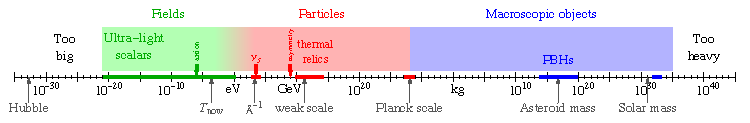
\includegraphics[width=\textwidth]{figs/MDMscale}$$
\caption[Range of DM mass]{\label{fig:DMrange}\em Possible {\bfseries range for the DM mass}, and some notable candidates. The edges of the shaded areas correspond to the lower and upper bounds in eq.~(\ref{eq:DMmassrange}).}
\end{figure}

\medskip

If DM is a particle with mass $M$, it will be located somewhere around the quantum mechanics boundary, possibly up to $M_{\rm Pl}$ which, as said above, is the limit for a particle. Empirically, the DM particle have to be heavier than $10^{-21}\eV \approx 10^{-49} M_{\rm Pl}$.
This lower limit is determined by the request that the de Broglie wavelength $R = 2\pi/Mv$ of a DM particle fits within the small gravitationally bound dwarf galaxies (which typically have kpc size, velocity $v \sim 10$ km/s, mass $\sim 5 \times 10^5 \, M_\odot$ where $M_\odot = 1.9984\times10^{30}$ kg is the solar mass) \cite{minimalM}.

DM can be heavier than the Planck mass, if it takes the form of a composite object, possibly up to the gravitational boundary
at which point black holes are the fundamental objects. In such a case, an upper bound is provided by the fact that the DM mass must be somewhat smaller than the mass of a typical small dwarf galaxy: since these have masses of the order of few $10^5 \, M_\odot$ (see section \ref{sec:dwarfs}), one can conservatively impose $M \lesssim 10^4 \, M_\odot$, to make sure that a sufficient number of DM `particles' inhabit the dwarfs.
It is worth emphasizing that the above absolute lower and upper limits of allowable DM mass $M$ arise from rather robust and model-independent considerations since they use just the basic properties of dwarf galaxies, the smallest astrophysical structures known to host Dark Matter. 

The `in-principle-viable' range of DM masses therefore  spans more than 90 orders of magnitude\footnote{One can similarly discuss the possible range for the strength of the interaction between DM and ordinary matter, which spans about 20 orders of magnitude from the minimal gravitational interaction $g \sim M/M_{\rm Pl}$ up to
strong-interaction-like couplings $g\sim 4\pi$. See Buckley and Peter~\cite{otherpastDMreviews} for the graphical representation of this range.}
\beq 
10^{-21}\eV < M < 10^{37}\kg.
\label{eq:DMmassrange}
\eeq
This huge range can be conceptually split in three main qualitatively different regions, illustrated in fig.\fig{DMrange}: fields, particles and macroscopic objects.
Fundamentally, particles and waves (fields) are the same objects, since 
Quantum Field Theory unifies them in a common description. 
 From a practical point of view, however, descriptions using particles or waves are different enough to be useful in different regimes (see section \ref{ultralight}).
As a rule of thumb, Dark Matter behaves as a classical field if $M \ll \eV$,
and as a particle if  heavier than the inverse Bohr radius $M \gg  \alpha m_e\sim  {\rm keV}$.
Dark Matter with de Broglie wavelength much smaller than atoms interacts with atoms individually, as a particle.
In the opposite limite DM undergoes collective interactions with ordinary materials.
The particle/wave transition similarly occurs in galaxies, where the observed DM density
can be reproduced by particles lighter than about an eV only if many quanta occupy the same phase space volume,
as we discuss shortly below. In this case DM can be described by a classical field. 
This is in complete analogy with electro-magnetism, where in the limit of many photons these are more simply described by classical electric and magnetic fields. Similarly, DM could be a massive boson that, in dense environments, is more simply described through a classical field.



\medskip

In other words, from the outset we do not  know whether DM physics belongs to astrophysics, particle physics or classical field theory.
The three possibilities are described in more details in the following sections:
\begin{enumerate}
\item Section~\ref{MACHO} and section~\ref{sec:DMmacro} discuss DM as composite objects heavier than the Planck scale. Primordial black holes are one possible candidate.
 \item Section~\ref{sec:DMparticle}  discusses DM as a new particle with mass $M$. In this case a plausible argument (see section \ref{sec:thermal_relic}) favors $M\sim \TeV$ --- the mass range currently explored by colliders and many other experiments --- but the possible candidate masses span many orders of magnitude below and above TeV.
\item Section~\ref{ultralight}  discusses DM as waves of ultra-light bosons, a possibility that is now also very actively investigated.
\end{enumerate}






\section{DM as very massive macroscopic objects}\label{MACHO}\index{Macroscopic objects}\index{DM!as super-massive}
DM could be made of Massive Astrophysical Compact Halo Objects (MACHOs\footnote{The name was coined in the early '90s (see K.~Griest (1991) in~\cite{MACHO}), in witty opposition to WIMPs, cf. section \ref{sec:WIMPs}.}), i.e.,\ ordinary astrophysical objects of macroscopic mass $M$, such as large planets, small dead stars or stray black holes \cite{MACHO}. These objects do not emit light and therefore fulfill the definition of dark matter. The MACHOs that are composed of baryonic matter {\em and} were created in the late Universe, like all the other astrophysical objects (the most natural expectation), require a large baryonic abundance, which contradicts the bounds from BBN and CMB discussed in section~\ref{sec:evidencesmaxi}.
DM made purely of {\em baryonic} MACHOs is thus ruled out. Nevertheless, it is still illustrative to consider their role as DM candidates, even though it is now mainly for historical reasons.

\medskip 


One way of identifying the presence of MACHOs in the Milky Way halo is via {\bf gravitational microlensing}. 
When a compact object with mass $M$ happens to cross the line of sight between the observer and a background star located at distance $L$,\footnote{More precisely, lensing occurs when the compact object is within a distance $\sim \sqrt{G M L}$ or less from the axis of the line of sight.} the light of such a star is lensed and its flux towards the Earth temporarily increases (two other related effects --- creating a second image or modifying the apparent size of the star --- are typically too small to be observable).

Since the time that MACHOs were first proposed in the '80s~\cite{MACHO} a number of surveys such as {\sc Eros-1}, -2, {\sc Macho}, {\sc Ogle}-I, -II, -III, -IV, tried to detect lensing signals by monitoring for several years millions of stars in the Magellanic clouds, which are  known environments that are relatively nearby, just outside our own Galaxy \cite{MACHOconstraints}. More recently, similar analyses  were performed with the {\sc Kepler} data, using local stars, and with the {\sc Subaru HSC} camera, using stars from the neighbouring galaxy Andromeda. 
The results by the {\sc Macho} collaboration in the year 2000 generated significant excitement, when it initially reported that between 8\% and 50\% of the mass in the Milky Way halo could be due to massive objects with preferred mass of about half $ M_\odot$. However, this possibility is excluded by other surveys which found only upper limits on $f$, the fraction of dark mass in the halo  that is in the form of massive objects.\footnote{An implicit assumption is that the fraction $f$ is the same in the whole Universe.} 
The recent reanalysis by \arxivref{2202.13819}{Blaineau et al.~(2022)}~\cite{MACHOconstraints} of archival data from the {\sc Eros-2} and {\sc Macho} surveys has focused on long duration microlensing events and has allowed to derive new constraints at large mass $M \gtrsim 10 \ M_\odot$. 
The recent results by \arxivref{2403.02386}{{\sc Ogle} (2024)} and \arxivref{2410.06251}{{\sc Ogle} (2024b)}~\cite{MACHOconstraints} combined about 20 years of observations as well as high-cadence observations and derived stringent bounds in the wide range $10^{-9} M_\odot \lesssim M \lesssim 10^{2} M_\odot$.
Combining the results of different campaigns gives
\beq\begin{array}{cc}
f \lesssim 5\% \quad \hbox{for} \quad 10^{-11}\, M_\odot \lesssim M \lesssim 100\, M_\odot \\
 \hbox{(exclusion by {\sc Eros, Ogle, Macho, Kepler, Subaru HSC})}.\label{eq:MACHO}
 \end{array}
\eeq
The detailed bounds are reported in fig.~\ref{fig:machos} (left). They hold under standard assumptions for the density and the distribution of the lensing objects, but could be weakened if, for instance, MACHOs are clustered (since this reduces the relative probability of them crossing a line of sight) or if their velocity dispersion is small. However, such effects are typically not sufficient to significantly weaken the bounds  (see \arxivref{1705.10818}{Green (2017)} in~\cite{PBHconstraints}).  
Other surveys, some still ongoing or upcoming, include {\sc Moa}, {\sc Super-Macho}, the Vera Rubin Observatory (formerly {\sc Lsst}), \dots~\cite{MACHOconstraints}.
That there are possible excesses of microlensing events was suggested by
\arxivref{1901.07120}{Niikura et al.~(2019)} and by
\arxivref{2009.04471}{Meneghetti et al.~(2020)} in~\cite{MACHOconstraints}.


\begin{figure}[t]
\begin{center}
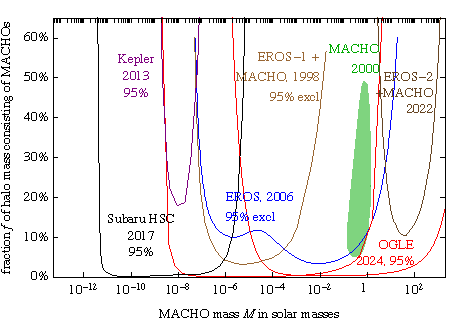
\includegraphics[width=0.48 \textwidth]{figs/machos} \hfill
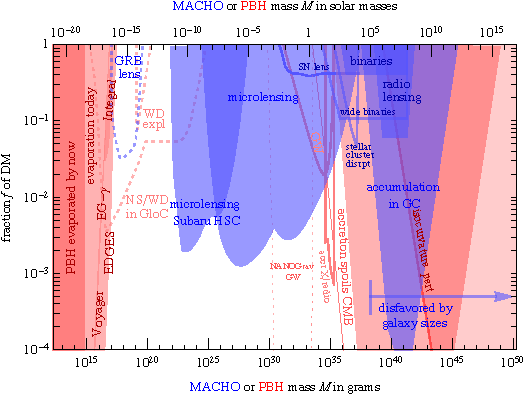
\includegraphics[width=0.48 \textwidth]{figs/pbhs} \end{center}
\caption[MACHO searches]{\em\label{fig:machos} {\bfseries MACHO searches}. 
{\bf {\em Left:}} Results of micro-lensing surveys (mostly towards the Magellanic Clouds): the bounds on the fraction $f$ of the Milky Way halo's mass which can be due to MACHOs, as a function of the object's mass $M$, as well as the region identified by the MACHO collaboration in 2000 (green). {\bf {\em Right:}} A collection of bounds on the fraction $f$ of DM consisting of massive astrophysical objects. The blue bounds apply to any MACHO, including Primordial Black Holes (PBH). The red bounds apply only to PBHs. The most recent or the most debated bounds are shown as dashed lines or as open (unshaded) contours. For a compilation of current constraints see also \href{https://github.com/bradkav/PBHbounds}{B. Kavanagh}, \href{https://doi.org/10.5281/zenodo.3538999}{PBHbounds}.}
\end{figure}

\medskip

Besides bounds from microlensing, there are also other constraints on MACHOs~\cite{MACHOconstraints}, a selection of which are given in fig.~\ref{fig:machos} (right). 
The non-observation of lensing effects in gamma ray bursts (femtolensing of GRBs) was originally used to disfavor MACHOs in the mass range $5\times10^{-17} - 2.5\times10^{-14}\, M_\odot$. This conclusion has  been disputed  by 
\arxivref{1807.11495}{Katz et al.~(2018)} and then \arxivref{1701.02151v3}{Niikura, Takada, Yasuda et al.~(2019)}~\cite{MACHOconstraints}, who pointed out that for these small MACHO masses the wavelength of the incoming light is larger than the Schwarzschild radius of the lensing object. This means that the diffraction due to the wave properties of light needs be taken into account and the geometrical optics approximation used in the original GRB studies becomes invalid. For the same reason the {\sc Subaru HSC} microlensing constraints cannot probe MACHOs with masses below $\sim 10^{-11}\, M_\odot$.
For much higher masses, the absence of lensing in the direction of type-Ia supernov\ae \ (SN-Ia) is claimed to exclude a large portion between $10^{-3} - 10^4 \, M_\odot$, however, this claim is also disputed.
At even higher MACHO masses, the absence of lensing for compact radio sources excludes the mass range $10^6 - 10^8\, M_\odot$. 

Very massive MACHOs are subject to many other constraints due to possible dynamical effects. Requiring that the binary star systems observed in the Galaxy are not disrupted by encouters with MACHOs rules out a mass range $10^3 - 10^8\, M_\odot$. The constraint extends to $10^{10}\, M_\odot$ (not shown in fig.~\ref{fig:machos}), if the survival of globular clusters is taken into consideration as well. Recent results on wide halo binaries even lower the bound to $10 \ M_\odot$. In a similar spirit, requiring that the stellar clusters observed at the center of ultra-faint dwarf galaxies, in particular Eridanus II, are not disrupted by the passage of MACHOs can impose a bound that, in its most conservative version, rules out a portion above $100\, M_\odot$ 
(recent simulations strengthen that to about $1\, M_\odot$, see \arxivref{2403.19015}{Koulen et al.~(2024)} \cite{MACHOconstraints}). 
Imposing that the amount of MACHOs being dragged (along with the stars) by dynamical friction into the galactic center region (see section \ref{sec:DynamicalFriction}) does not exceed the observed mass of the GC region itself, disfavors the large portion around $2 \times10^4 - 10^{12} M_\odot$. This constraint is sensitive to the details of galactic dynamics, though. For instance, an in-falling MACHO could kick stars or other MACHOs out of the GC via gravitational slingshot effects, reducing the accumulation rate. Another bound excluding MACHOs with masses $10^4 - 10^{10}\, M_\odot$ (not shown in fig.~\ref{fig:machos}) comes from requiring that DM behaves like a fluid, and not as a collection of discrete massive objects, in the formation of Large Scale Structures.
Finally, the very heavy MACHOs in fig.~\ref{fig:machos} (right) are highly disfavored simply because a single DM `particle' cannot be heavier than the smallest of the objects formed by DM particles, as discussed around eq.~(\ref{eq:DMmassrange}): the sizes of dwarf galaxies such as Segue 1 ($\sim 5\times 10^5\, M_\odot$) or even of the Milky Way ($\sim 5\times 10^{11}\, M_\odot$) arguably impose robust upper bounds on MACHO masses, unless one is willing to allow tailor-made MACHOs for each galaxy... More stringent bounds could be derived by imposing that a sizable number of DM `particles' must constitute the halos of these objects (to avoid granularities) or by detailed modelling of even smaller bodies (e.g., globular clusters).

\medskip

In summary, the various observational and dynamical bounds only leave open the region at small MACHO masses ($M \lesssim 3 \times 10^{-12} M_\odot$). 
If the  bounds from supernova lensing, the wide binaries and Eridanus II are discarded, and before the recent extension of the bounds using archival data from the {\sc Eros-2} and {\sc Macho} surveys, the region of MACHO masses around 10 to 400 $M_\odot$ was viable as well. The latter possibility attracted significant attention in the wake of the gravitational wave detection by {\sc Ligo}, as we mention in the following subsection. \\
However, let us recall: all of the above discussion is subject to the fact that the BBN and CMB constraints contradict the existence of baryonic bodies of astrophysical nature, of any mass, as an explanation for DM abundance, if these formed after the BBN.


\subsection{Primordial black holes}\label{sec:PBHs}\index{Primordial black holes}\index{DM!as black holes}\index{Black hole!as DM}
Astrophysical objects that consist of baryonic matter, but have somehow been created {\em before} the BBN, are not subject to the cosmological constraints of section~\ref{sec:evidencesmaxi}, since the material that they are made of gets subtracted  from the baryonic budget very early on. This is the case with {\em primordial} black holes (PBHs)~\cite{PBH}.\footnote{An interesting questions is whether one can distinguish observationally a Primordial BH from a standard BH created in a stellar collapse (e.g.,~via the signal of gravitational waves emitted in BH mergers). In principle, there are several possibilities: i) detection of a BH with a mass smaller than about $3M_\odot$ would imply that a PBH was observed, since astrophysics predicts that for such light objects the gravitational collapse is stopped by neutron degeneracy pressure and a neutron star is born (for a nonstandard exception see~\cite{1804.06740}); ii) detect a BH at very high redshift (say, $z > 8$), an epoch before the birth of first stars; iii) find evidence for a spatial distribution of BHs not correlated with the galactic disks.}
PBH formation mechanisms will be discussed in section~\ref{sec:PBHform}, and possible underlying theories in sections~\ref{sec:BHth}, \ref{sec:BHth2} and \ref{sec:PBHSM}. Here we discuss their viability as DM candidates.




\medskip
Several {\bf phenomenological constraints} apply to PBHs as candidates for DM~\cite{PBHconstraints}, shown in fig.~\ref{fig:machos} (right). First of all, the bounds on MACHOs discussed in section~\ref{MACHO} rely only on their gravitational pull and thus also apply to PBHs.
 
An additional condition is that the PBHs should not have evaporated by now. Quantum fluctuations of fields around any black hole lead to the emission of {\em Hawking radiation}, a thermal spectrum of particles at a temperature\footnote{Although the phenomenon of BH Hawking radiation has never been confirmed observationally, there are strong theoretical and experimental arguments in its favor (for instance, the equivalent of a Hawking radiation was observed in fluido-dynamical systems that share some properties with the BHs). 
Let us however note that several recent works 
suggested that Hawking evaporation slows down or even stops as the BH's mass decreases, due to a quantum memory burden effect~\cite{memoryburden}. 
If this were indeed the case, evaporation constraints would no longer apply or at the very least would be relaxed over vast portions of the parameter space, which would thus be allowed again.\index{Primordial black holes!memory burden} Note also that the effect implies that two BH with the same mass would evaporate at different rates, if they have a different past history, contradicting the `no-hair' principle.
Other conditions in which Hawking radiation is argued to be slowed down or stopped are rotating (and/or electrically charged) BH, as well as BH in extra-dimensional spaces \cite{noHawkingRad}.
Finally, let us mention that, according to~\cite{2401.14431}, the gravitational collapse of objects with higher central density might give rise to
{\em primordial naked singularities}, that could behave as DM similarly to PBH, but without emitting Hawking radiation.}
\beq \bbox{T_{\rm BH}=1/(8\pi  G M)}~.\eeq
The total radiated power is  $W \approx g\, 4\pi R_{\rm Sch}^2 \sigma T_{\rm BH}^4=g/(15360\, \pi\, G^2 \, M^2)$
where $g$ is the number of degrees of freedom lighter than $T_{\rm BH}$,
$\sigma=\pi^2/60$ is the  Stefan-Boltzmann constant and $R_{\rm Sch}=2GM$ the Schwarzschild radius.
The BH loses mass at the same rate, $\dot M = - W$, so that within time 
\beq \tau_{\rm BH} \approx 5120\,\pi \, G^2  M^3/g,\eeq
the BH fully evaporates. 
Evaporation happens when the age of the universe is comparable to $\tau_{\rm BH}$,
corresponding to the cosmological temperature $T_{\rm ev} \sim M_{\rm Pl} ^{5/2}/M^{3/2}$.
Requiring that the PBH's lifetime is longer than the age of the Universe implies $T_{\rm ev}\circa{<} T_0$, where $T_0\simeq 2.7\,$K is the current CMB temperature, so
\beq M \gtrsim M_{\rm Pl}^{5/3}/T_0^{2/3}\sim
10^{-19}\, M_\odot . \eeq
A detailed computation gives $M > 2.5\times 10^{-19}\, M_\odot$.\footnote{
 A possible loophole to this argument occurs if PBHs evaporate via Hawking radiation, 
 but then leave behind {\em stable Planck-mass relics}, 
 which do not evaporate further. Such remnants could constitute the DM~\cite{PlanckRelics} 
 (as long as the last stages of the evaporation do not provide them with a momentum kick that would make them non-cold, as argued in some models). With an estimated cross section of 
 $1/M_{\rm Pl}^2 \sim 10^{-66} \,{\rm cm}^2$, 
 they would be essentially inert and undetectable (other than by their gravitational effects, see section~\ref{gravisignal}). It has also been argued that the relics could carry an electric charge, if evaporation halts abruptly in a non-zero-charge configuration.  \index{DM properties!charge}
This possibility is strongly constrained, see section~\ref{sec:milicharged}. 
Alternatively, doubts related to unitarity suggest that after some time the semiclassical approximation that leads to
Hawking radiation could fail, and maybe the BH lifetime is much longer than $\tau_{\rm BH}$.}
PBHs with a mass slightly above this value would be in the process of evaporating at the present time, emitting particles with a temperature of around 80 MeV. The non observation of such Hawking radiation, e.g. in the extragalactic $\gamma$-ray flux or in the flux of low energy electrons and positrons measured by the {\sc Voyager-1} spacecraft outside of the solar system, imposes the more stringent bound $M \gtrsim 4\times 10^{-17}\, M_\odot$. 
In addition, the emitted low energy $e^\pm$ would diffuse and annihilate. Requiring that the resulting contributions to the $X$-ray signal measured by {\sc Integral} are not too large extends the bound by a tiny bit to $M \gtrsim 6\times 10^{-17}\, M_\odot$.

Similarly, the evaporation of PBHs around the epoch of reionization would have heated up the intergalactic medium and weakened the 21cm absorption signal, claimed by the {\sc Edges} experiment. 
This provides a bound  around $M \sim 10^{-16}\, M_\odot$ (denoted as {\sc Edges} in fig.~\ref{fig:machos} right) and possibly around 10 $M_\odot$ (the latter, not shown in fig.~\ref{fig:machos} right, should not be confused with the bounds imposed by the CMB due to accretion, discussed two paragraphs below).
The heating of the intergalactic medium can also be constrained via the Lyman-$\alpha$ forest and by its effect on the CMB anisotropies as observed on Earth. These effects provide limits around $M \sim 10^{-16}\, M_\odot$ similar to the {\sc Edges} one, hence for simplicity we do not report them in the figure.


\index{Neutron star}\index{White dwarf}
Constraints based on the survival rates of neutron stars (NS) of white dwarfs (WD) in Globular Clusters (GloC) apply to the PBH masses in the range
from  $10^{-18}\, M_\odot$ to $10^{-9} \, M_\odot$. Such PBHs could sink to the interior of NS/WD, either during the formation of the NS/WD or by subsequent capture, and quickly destroy them by eating them from the inside. The mere observation of existing neutron stars and white dwarfs then imposes the constraint on PHBs. However, such bounds rely on the assumption of a very large density of DM in Globular Clusters (of the order of $10^3$ GeV/cm$^3$ and higher), which is far from certain. For this reason the bound is indicated as an open dashed contour in fig.~\ref{fig:machos}.

Using similar physics, the PBHs in the mass range between $5\, 10^{-15} \, M_\odot$ and $10^{-13} \, M_\odot$ were claimed to be excluded based on the fact that PBHs piercing the bodies of white dwarf stars (WD) could heat the stellar matter and trigger the death of WDs in a form of supernova explosions at a rate higher than observed.
However, more detailed numerical computations invalidated this bound. 

Another important point is the fact that PBHs, like any other BH, would accrete material. 
On the one hand, this could help explain why some dense structures are heavily dominated by DM: the PBHs may have swallowed a lot of the baryonic material early on, eventually penalizing the star formation, as argued by \arxivref{1711.10458}{Clesse \& Garc\'ia-Bellido (2018)}~\cite{PBH}.
On the other hand, the infalling gas would emit $X$-rays, which would ionize matter, and thus affect the observed CMB spectrum and anisotropies. 
This rules out a very large range of PBH masses around  $10^2 - 10^{16}\, M_\odot$.\footnote{The early computation in \arxivref{0709.0524}{Ricotti et al.~(2007)}~\cite{PBHconstraints}, which found more constraining bounds down to $10^{-1}\, M_\odot$, was later revisited and the bound relaxed.} By refining the accretion model, \arxivref{1707.04206}{Poulin et al.~(2017)}~\cite{PBHconstraints} improved the exclusion on the low mass end by about 2 orders of magnitude (open pink contour in fig.~\ref{fig:machos} right). 
The same $X$-ray (and radio) emissions from accretion should be visible if PBHs are present in our Galaxy. 
Their non-observation 
imposes a bound in the PBH mass window from a few $M_\odot$ to $100 \, M_\odot$ and possibly beyond.
Importantly, all these bounds are subject to the uncertainties related to the modelling of the accretion process, which in itself  is an active area of research in astrophysics, and by no means a settled subject, especially in the conditions encountered for  
these BH masses ($1-100\, M_\odot$), gas densities ($\gtrsim 200$ particles/cm$^3$ at CMB formation) and relative PBH/gas speeds (super- or sub-sonic depending on the models).

Incidentally, the $10 - 100 \, M_\odot$ mass interval attracted a lot of attention in the wake of the {\sc Ligo} gravitational wave events~\cite{1602.03837}, which have been advocated by some groups to be due to mergers of PBHs~\cite{PBHandLIGO}. However, for PBHs with such masses to be viable DM candidates the bounds from long duration lensing events in {\sc Eros-2} and {\sc Macho}, from accretion, from SN lensing, from wide binaries and possibly from CMB distortions and stellar cluster disruptions in Eridanus II would all have to be dismissed. 
A few works \cite{PBHandLIGO}  instead used the same {\sc Ligo} observations, along with the estimates of PBH merger rates, to derive the exclusion contours shown in fig.~\ref{fig:machos}  with the GW label (note, though, that the existence of such bounds has been questioned by others).
An even wider range of masses ($3 \times 10^{-4} M_\odot < M < 2 M_\odot$) was claimed to be strongly excluded by the fact that {\sc NANOGrav} has not  yet detected gravitational waves, even though these should in principle have been  produced at the same time as the PBHs were created. The exclusion relies on extreme assumptions about the PBH production mechanism, has been questioned in the literature, and we thus show it 
as a dotted contour in fig.~\ref{fig:machos}.

Finally, all the large range above $5 \, 10^{6} \, M_\odot$, already disfavored by the size of galaxies and other MACHO bounds discussed above, is ruled out by the fact their discreteness would induce isocurvature perturbations in contrast with the CMB measurements, as argued by \arxivref{2508.08238}{Gerlach et al.~(2025)}~\cite{PBHconstraints}.



\medskip

In summary, being very conservative when taking into account the constraints for different ranges of PBH masses, we find that
at the time of writing the PBHs could constitute the whole of Dark Matter ($f=1$) for
\begin{equation} 
 \bbox{10^{-16}\,  M_\odot \lesssim M \lesssim 3\times10^{-12}\, M_\odot. }
 \label{eq:PBH}
\end{equation}
Black holes at the low end of this range would have radii smaller than the size of an atom and mass comparable to a small asteroid or Mount Everest. On average, roughly one such PBH would be expected to be present in the volume of the solar system.
Also note that many of the bounds are still under active discussion, as mentioned above, so that the situation could well change. 


\medskip

It is important to stress that the above results apply under a couple of important simplifying assumptions. The first one is that all the PBHs have the same mass, i.e.,~a `monochromatic mass function'. In the more general, and probably more realistic, case in which the PBHs masses are distributed according to an {\bf extended mass function}, each mass could in principle lie below the various constraints and they could sum up to the needed total amount. The analysis is however complex since the monochromatic bounds cannot be applied straightforwardly, the constraints need to be re-evaluated at all the masses included in the specific mass function. Current results seem to indicate that PBHs with some extended mass functions (e.g.~lognormal) might still account for the whole of DM in some restricted windows~\cite{PBHextendedmassfunction}.
As discussed in section~\ref{sec:BHth}, many mechanisms can give rise to PBHs masses that span about an order of magnitude.



The second simplifying assumption is that PBHs are homogeneously distributed in space. If they instead wander around in the galactic halo grouped in {\bf clusters}, as their formation history might suggest, the bounds might be affected. On the one hand, the lensing limits are expected to be relaxed, since the cluster
tends to behave as a single lensing body of larger mass than the constituent PBHs, therefore falling `to the right' of the region in mass probed by the lensing surveys. 
CMB limits could also be loosened, since the high proper velocity of the PBHs within the cluster implies a less efficient accretion.
On the other hand, the tight packing inside clusters is expected to favour merging events, 
therefore enhancing the emitted signals in gravitational waves and strengthening the corresponding constraints. 
The extent to which clustering occurs and its detailed impact on the different bounds are subjects of active investigations~\cite{PBHclustering}.


\medskip

One can also imagine more complicated scenarios. For instance, some works explored a hybrid hypothesis, where the total DM abundance would be a mix of PBHs and particle DM (possibly produced by the PBHs themselves via evaporation), in varying proportions~\cite{PBHsandWIMPs}. 
However, quite often the two are  mutually exclusive. For instance, in the hybrid scenario where DM are WIMPs,  see section~\ref{chapter:indirect},  the WIMPs would accumulate around PBHs and tend to produce a DM annihilation signal (see section \ref{sec:DMBH}) incompatible with observations. 
The DM abundance must in that case be either predominantly due to PBHs or predominantly due to WIMPs,
see e.g.\ \arxivref{2011.01930}{Carr, Kuhnel \& Visinelli (2020)} in~\cite{PBHsandWIMPs}.



\medskip

Future prospects to further explore the PBH parameter space include the following ideas~\cite{PBHperspectives}.
For  low mass window, $M \lesssim 10^{-12} M_\odot$, the stochastic background of gravity waves emitted during formation of PBHs is expected to be within the sensitivity of the future (2037?) space interferometer {\sc Lisa}, but with the caveat that the astrophysical backgrounds are still highly uncertain (see, e.g.,~\arxivref{1811.08797}{Christensen (2018)} in \cite{PBHperspectives}).
Similar masses can be tested by detecting the seismic oscillations that a PBH would produce when piercing the body of the Sun or another star (or even the Earth, an event which would, somewhat anticlimactically, only result in a small albeit peculiar earthquake) or neutron stars.
Sensing the motion of passing PBHs in the Galaxy via the modification to the timing of the signal of a pulsar could allow to test the $10 - 100 \, M_\odot$  {\sc Ligo} range. Using pulsar timing arrays (PTA) could probe a much larger mass window: \arxivref{1901.04490}{Dror et al.~(2019)} estimate that future PTA observations with the Square Kilometer Array ({\sc Ska}) may probe the range $10^{-12} \, M_\odot \lesssim M \lesssim100 \, M_\odot$; 
the current {\sc NanoGrav} results only constrain $f\lesssim 300$ on the range $10^{-6} \, M_\odot \lesssim M \lesssim10^{4} \, M_\odot$ \cite{PTA}.  




\section{Dark Matter as macroscopic objects}\label{sec:DMmacro}\index{Macroscopic objects}\index{DM!as macroscopic}
DM heavier than the Planck mass $M_{\rm Pl}\approx 2\, 10^{-5}\,{\rm gram}$ 
and lighter than the quasi-stable black holes,
$M_{\rm Pl}^{5/3}/T_0^{2/3} \sim 10^{15}\,{\rm gram}$,
might exist if sub-Planckian particles form composite objects with macroscopic mass~\cite{MacroscopicDM}.
We assume a common mass $M$ and cross section $\sigma$ for scattering on matter, usually rewritten as $\sigma = \pi R^2$.
In many models  $R$ is the radius of the object, but more generally it can be a parameter of the theory, only alluding to the geometrical meaning.
The two parameters $M$ and $R$ then determine the phenomenology.
Detecting such candidates is difficult because they are very rare: their flux
$\Phi = \rho v/4\pi M$ is suppressed by the large mass $M$.
As a result, their impact rate (in one direction) on a target with area $A$ is
\beq 
\Gamma =\frac{\rho_{\odot} vA}{4M} \approx \frac{1.6}{\rm yr} \frac{\rm g}{M} \frac{A}{\km^2},
 \eeq 
where in the numerical estimate we assumed the local DM density $\rho_{\odot}=0.4\GeV/\cm^2$ (see eq.~(\ref{eq:rhosun:value})) and velocity $v =10^{-3} c$ (see eq.~(\ref{eq:rms:v0})). 
 Assuming that in the scattering events the macroscopic object
 only releases its kinetic energy\footnote{More speculative macroscopic objects made of anti-matter would annihilate, releasing more energy.} the bounds, plotted in fig.\fig{MacroCompositeDM}, are as follows.

\begin{figure}[t]
$$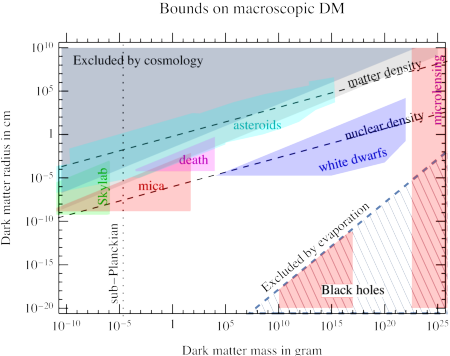
\includegraphics[width=0.7\textwidth]{figs/MacroCompositeDM}$$
\caption[Macroscopic DM]{\label{fig:MacroCompositeDM}\em DM is here assumed to be a {\bfseries macroscopic object} with mass $M$
and radius $R$, describing a cross section on matter $\sigma \approx \pi R^2$.
Shaded regions are  bounds from cosmology, Skylab, ancient mica, sudden death by DM, micro-lensing, 
collapse of white dwarfs, formation of black holes
and their evaporation~\cite{MacroscopicDM}.
The dashed lines correspond to object with the density of normal matter or of nuclear matter.
}
\end{figure}

\begin{itemize}
\item[$\circ$] A $\m^2$ area inside the Skylab space station has been monitored for a yr, 
giving the bound $\Gamma \circa{<} 1/ \ {\rm m}^2\yr$ that excludes barely sub-Planckian $M$.
However, the bound only applies if  $\sigma\circa{>} 10^{-18}\cm^2$  (as needed to detectably damage the material)
and if $\sigma/M\circa{<}3\cm^2/\gram$ (as needed to enter the Skylab).
The combination of these considerations gives the exclusion region shown in fig.\fig{MacroCompositeDM}.

\item[$\circ$] The lack of tracks in 500 Myr old mica gives the bound at $M \circa{>}55\gram$ if again $\sigma\circa{>} 10^{-18}\cm^2$ 
(needed to damage mica) and if $\sigma/M <3~10^{-6}\cm^2/\gram$ (such that DM reached mica underground).

\item[$\circ$] Similarly, the lack of people killed by impacts with DM 
gives the bound $M \circa{>}10\,{\rm kg}$ if $\sigma\circa{>} 10^{-8}\cm^2$ 
(needed to deposit as much energy as a bullet) and if $\sigma/M \circa{<}10^{-4}\cm^2/\gram$
(such that energetic DM reaches Earth's surface).

\item[$\circ$] In a similar spirit, the lack of evidence for the destruction of asteroids and other similar bodies such as those composing the rings of Saturn, or for significant displacements from their orbits, excludes the area in cyan in fig.\fig{MacroCompositeDM} (see \arxivref{2504.07232}{Picker (2025)} in \cite{MacroscopicDM}).   

\item[$\circ$] Cosmology gives the bound $\sigma/M \circa{<} 3~10^{-3}\cm^2/\gram$ on dark-matter interactions with baryons,
and $\sigma/M \circa{<} 5~10^{-7}\cm^2/\gram$ on dark-matter interactions with photons.

\item[$\circ$] Very heavy DM would produce unseen micro-lensing effects if $M\circa{>}2~10^{22}\gram$ (see section \ref{MACHO}).

\item[$\circ$] Macroscopic DM could heat white dwarfs, igniting thermo-nuclear runaways.
The existence of long-lived white dwarfs excludes the region in blue in fig.\fig{MacroCompositeDM}~\cite{MacroscopicDM}.
Its complicated shape arises from requiring the DM heating rate to be bigger than the cooling rate, 
 and that DM is able to penetrate the external layers of a white dwarf.

\end{itemize}


Possible theories of cosmological formation of
DM as macroscopic objects are discussed in section~\ref{sec:MacroCompositeDMth}.


\section{Particle Dark Matter}\label{sec:DMparticle}\index{Particle DM}\index{DM!as particles}
The most studied possibility is that DM is made of particles. A viable particle DM candidate must have the following properties (rephrasing the properties listed in chapter \ref{sec:evidences} in particle physics term):

\begin{enumerate}
\index{DM properties!cold}
\item DM must be {\em cold} or at least {\em not too hot}. Technically, this means that DM needs to be non-relativistic at the time that structures start to form, somewhat before matter-radiation equality at $z \sim 3400$,
%(occurring in turn just before photon decoupling, i.e., at the time of~CMB formation, $z \sim 1100$), 
and henceforth during all the subsequent periods of galaxy formation, as discussed in section \ref{sec:linear:inhom}. 
This means that the typical velocity of DM particles, $v$, is much smaller than the speed of light, $v \ll c$, or, equivalently, that their typical momentum, $p$, is much smaller than their mass, $p \ll M$.
If DM is made of thermalized particles, this implies that they must be heavier than a few keV, as we discuss in section~\ref{sec:WarmDM}.
\index{DM properties!charge}
\item  The {\em electric charge $q$} of a DM particle must be {\em null or very small}.
The experimental bounds on the allowed values reach $q\circa{<}10^{-10}$ for DM with a weak scale mass, $M\circa{<}\TeV$.  For heavier DM the bounds become gradually weaker, reaching $q\circa{<}0.3$ for  Planck mass DM (the bounds are summarized in fig.\fig{chargedDM}). For $q\simeq 10^{-11}$ the freeze-in mechanism (see section \ref{Freeze-in}) gives the correct relic abundance almost irrespective of DM mass, a possibility that is not experimentally excluded. We expand on some of the details concerning the (milli-)charged DM in section \ref{sec:milicharged}.





\item  Bounds from direct detection experiments, discussed in section~\ref{chapter:direct}, imply that
{\em the cross section for scattering of DM on normal matter is smaller than a typical weak cross section},
 $\sigma \ll 1/M_Z^2$, for $M \sim M_Z$.
The bound on $\sigma$ becomes much less constraining for $M \ll \GeV$, and becomes less constraining also for $M \gg M_Z$, in which case it scales as $M/M_Z$. 
Among other things this means that the possible DM coupling to the $Z$ boson must be significantly smaller than a typical weak interaction
for DM lighter than $\sim 10^7\TeV$.


\index{DM properties!non-interacting}
\item  The {\em cross section among two DM particles} must be {\em smaller than a typical QCD cross section}, 
$\sigma/M \ll  (\GeV/M)/M_\pi^2$, where $M_\pi=135$ MeV  is the pion mass. This bound is easily satisfied for particles that do not have strong interactions.
For larger cross sections DM would not have behaved as a collision-less fluid in cosmology and in astrophysical systems. We discuss the possibility of self-interacting DM in section~\ref{sec:SIDM}.

\index{DM properties!stable}
\item The DM particle must be {\em stable}, or have a lifetime much longer than the age of the Universe ($\approx 13.8$ Gyr = 4.35  $10^{17}$ s) so that the cosmological effects of DM decays are negligible.
If DM had decayed too early, it would not have played its important role in shaping the Large Scale Structures of the Universe and/or we would have observed its decay products. Current limits on DM lifetime are of the order of $\tau \gtrsim 10^{28}$ s (see, e.g.,~fig.~\ref{fig:IDconstraintsdecay} in section \ref{sec:IDconstraints}).

\end{enumerate}

\renewcommand{\arraystretch}{0.7}
\begin{table}[!t]
\begin{center}
\small{
\begin{tabular}{c|c|c|c}
\bf Candidate & \bf Date & \bf Reference(s) & \bf  Section \\[1mm]
\hline 
 & & & \\[-1mm]
Primordial BH 		& 1966, 1971 & Zeldovich \& Novikov, Hawking \cite{PBH} & \ref{sec:PBHs} \\[1mm]
MACHOs	 		& 1981, 1986 & Petrou; Paczynski \cite{MACHO} & \ref{MACHO} \\[1mm]
\hdashline 
 & & & \\[-2mm]
Gravitinos			& 1981, 1982 & Fayet; Witten; Pagel \& Primack \cite{gravitinoDM} & \ref{sec:gravitinoDM} \\[1mm]
Axions 			& 1983 & Preskill, Wise \& Wilczek \cite{axionDM} & \ref{axion} \\[1mm]
Neutralinos 	& 1984 & Ellis et al.~\cite{SuSyDM} & \ref{SUSY} 
\\[1mm]
Strangelets		& 1984 &  Witten; Fahri \& Jaffe \cite{quark:matter:DM} & \ref{sec:quarkmatter} \\[1mm]
$Q$-balls			& 1984 &  Witten \cite{QballsBis} & \ref{sec:Q} \\[1mm]
Extra-dimensional DM & 1984 & Kolb \& Slansky; Servant \& Tait \cite{xdimDM} & \ref{sec:Xdim} \\[1mm]
WIMPs 			& 1985 & Steigman \& Turner \cite{WIMPs} & \ref{sec:WIMPs} \\[1mm]
Sterile neutrinos	& 1993 & Dodelson \& Widrow \cite{SterileNu} & \ref{FermionSinglet} \\[1mm]
Fuzzy DM 		& 2000 & Hu, Barkana \& Gruzinov \cite{FuzzyDM} & \ref{ultralight} \\[1mm]
Sub-GeV DM		& 2003 & Boehm, Fayet et al.~\cite{sub-GeVDM} & \ref{unitarity} \\[1mm] 
\end{tabular}}
\end{center}
\vspace{-5mm}
\caption[Historic particle DM candidates]{\em\label{tab:candidates} {\bfseries Some historic DM candidates} (mostly in the particle DM category) or classes of candidates.}
\end{table}
\renewcommand{\arraystretch}{1}

In section~\ref{SMDM} we will see that
the above properties are not simultaneously satisfied by any of the Standard Model particles. 
As a consequence, new unknown and so far undiscovered kinds of fundamental particles are invoked (see table \ref{tab:candidates}),
as discussed in chapters~\ref{models}, \ref{BigDMtheories}.


\medskip

Note that the above list does not specify anything about the mass of the DM particle: as long as one does not commit to a specific model or a specific production mechanism, DM particles can be as light as 1 eV or as heavy as $M_{\rm Pl}$ (the edges of the `particle realm' in eq.~\ref{eq:DMmassrange} and in figure \ref{fig:DMrange}). DM can consist of a very large number of very light particles or, alternatively, of a much smaller number of much heavier particles, or anything in between, where all these possibilities are  compatible with all the observations.  
The allowed range of DM masses does depend, though, on whether the DM particle is a fermion or a boson. 
Fermionic DM is subject to the Pauli exclusion principle, which leads to a lower bound on DM mass, first derived by\index{Gunn \& Tremaine bound}\index{Bounds!Gunn \& Tremaine}
{\bf Gunn and Tremaine}~\cite{GunnTremaine}.
For concreteness, let us consider the Milky Way, where the local DM density is 
$\rho_\odot \approx 0.4\GeV/\cm^3 \approx (0.04\eV)^4$
and the galactic escape velocity is $v_{\rm esc} \approx 10^{-3}$.
The de Broglie wave-length is $\lambda =2\pi/Mv$, where $v$ must be smaller than the escape velocity.
Assuming a single DM fermion species, its quantum occupation number is required to be smaller than one.
The maximal DM density is therefore $\rho \circa{<} M/\lambda^3$, which implies
$M\circa{>}1\keV$. Note that throughout this argument we were able to treat DM fermions as free, given the
bounds on DM self-interactions (see section~\ref{sec:SIDM}). 
More precisely, a  detailed study of dwarf spheroidal galaxies finds~\cite{GunnTremaine}
\beq 
\label{eq:GunnTremaine}
M>0.1\keV  \qquad {\rm (fermionic} \ {\rm DM).}
\eeq
This bound is robust and independent from the model of DM formation and DM decoupling.
It gets relaxed by a factor $N^{1/4}$, if there are $N$ independent fermion species;
bounds on their gravitational production at colliders allow up to $N \circa{<}10^{60}$~\cite{GunnTremaine}.
The bound in \eqref{eq:GunnTremaine} implies, in particular, that the Standard Model neutrinos cannot be the DM, as discussed in more detail in section~\ref{neutrinoDM}.

Bosonic DM is not subject to the above bound and can be much lighter. 
In other words, DM lighter than 0.1 keV must be bosonic. 
In fact, bosonic DM particles can be so light that this brings us outside the domain of particle DM,
as discussed in section~\ref{LightBosonDM}.


\subsection{Warm DM}
\label{sec:WarmDM}
\index{Warm DM}\index{DM properties!warm}

DM made of particles with negligible velocity is dubbed {\em cold DM};
{\em hot DM} refers to quasi-relativistic DM particles,
and {\em warm DM} (WDM) to the intermediate regime \cite{WarmDMhistory}.
As shown in section \ref{sec:linear:inhom}, hot DM is excluded by structure formation.
SM neutrinos would qualify as hot DM, and thereby cannot be the DM (see section \ref{neutrinoDM}). 
The intermediate situation is intriguing since the moderate motions of WDM particles smoothen out structures on small cosmological scales (e.g.~dwarf galaxies or the cores of galaxies) and could alleviate some of the potential problems with cold DM, see section~\ref{sec:astroanomaly}. Indeed, this possibility is so interesting that  numerical simulations including WDM have been performed by a number of groups \cite{Sims_alt_DM}.\index{Numerical simulations!warm DM}

\smallskip

Quantitatively, the observable of interest is the free-streaming length of DM particles at the beginning of structure formation: any structures smaller than this length get  washed out.
Lyman-$\alpha$ data (i.e. the analysis of absorption inside hydrogen clouds of the light emitted at the Lyman-$\alpha$ frequency from a background source, such as a quasar) allow to probe the distribution of matter on small scales and therefore to test DM free-streaming.
Barring possible anomalies, Lyman-$\alpha$ observations agree with CDM and
constrain warm DM to be heavier than a few keV: the lighter the DM, the hotter it tends to be.
More precisely, this bound is weaker if in the early universe DM was produced via some non-thermal mechanism with energies lower than those of the SM plasma.
In principle, the bound depends on the full DM velocity distribution.
In practice, however, the bound on the DM mass $M$ can be well approximated using the average momentum-to-temperature ratio $\langle p/T\rangle$, giving~\cite{WarmDMbounds}
\beq 
\bbox{
M \circa{>} 1.9\keV \, {\left\langle \frac{p}{T}\right\rangle_{\rm prod}}
\left(\frac{106.75}{g_{\rm SM}(T_{\rm prod})}\right)^{1/3}}~.
\label{eq:WarmDMbounds}
\eeq
Different groups obtain similar bounds, affected by astrophysical uncertainties.
Above, the number of SM degrees of freedom $g_{\rm SM}$ were normalized to its
maximal value, 106.75, which is reached for $T_{\rm prod} \gg M_Z$. The DM velocity factor $\langle p/T\rangle $ entering \eqref{eq:WarmDMbounds} is determined either by the moment at which DM decouples (if DM was already present in the plasma in thermal equilibrium), or at the moment DM is predominantly produced (out of equilibrium). We mark this moment by the temperature of the SM bath, $T= T_{\rm prod}$.
In the subsequent cosmological evolution the $p/T$ ratio changes only when entropy is injected into the SM plasma,
giving at lower temperatures $\med{p/T} = \med{p/T}_{\rm prod} [g_{\rm SM}(T)/g_{\rm SM}(T_{\rm prod})]^{1/3}$, explaining the form of the last two factors in eq.~\eqref{eq:WarmDMbounds}.


The DM velocity factor at production 
equals ${\langle p/T\rangle_{\rm prod}} = 3.15$, if DM is a fermionic species that underwent 
relativistic freeze-out;
3 in the Boltzmann approximation;
higher if DM is a sterile neutrino produced via oscillations;
$2.45$ if DM is produced from decays of a much heavier thermalized scalar;
lower if DM is produced by decays of a slightly heavier particle such that the phase space is partially closed. 
Bosonic DM  can evade the above bounds by
developing a classical condensate with negligible $p/T$ (section~\ref{LightBosonDM}).

\medskip

Lyman-$\alpha$ observations are not the only way to probe the distribution of matter at small scales and therefore test WDM. Another technique involves the observations of strong gravitational lensing events in order to reconstruct the distribution of the intervening matter. One can also consider the number of Milky Way satellites predicted (via numerical or semi-analytical methods) in presence of WDM and compare it with the counting performed by local surveys. 
The inferred bounds on the DM mass~\cite{WarmDMbounds} are in the same ballpark as eq.~(\ref{eq:WarmDMbounds}).

Historically, popular particle physics candidates that behave as warm dark matter 
 include sterile neutrinos (section \ref{FermionSinglet}) and gravitinos (section \ref{sec:gravitinoDM}) \cite{WarmDMhistory}.



\subsection{(Milli-)charged Dark Matter}\label{sec:milicharged}
\index{Charged DM}\index{Milli-charged DM}\label{DM properties!charge}

\begin{figure}
\begin{center}
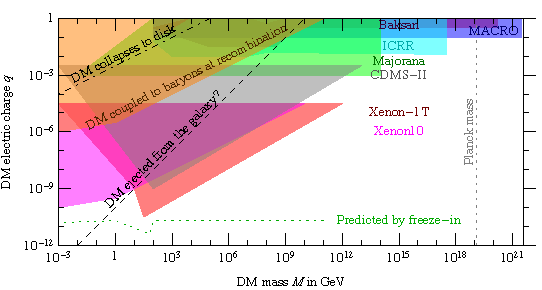
\includegraphics[width=0.75\textwidth]{figs/ChargedDM}
\caption[Charged DM]{\em Experimental bounds on a possible {\bfseries electric charge of DM}. Most of the bounds are reproduced from the references in \cite{CHAMP-exp}, but some are extended as discussed in the text.
\label{fig:chargedDM}}
\end{center}
\end{figure}

A simple possibility for DM to interact with the SM particles is for DM to carry small electromagnetic charge $q |e|$,
where $e=-1.6\ 10^{-19}\,{\rm C}$ is the charge of the electron~\cite{CHAMP}. This kind of particles are historically refereed to as CHAMPs, for Charged Massive Particles.
The charge $e$ is a convenient unit  since in plausible 
contexts, such as the SU(5) gauge unification, uncolored particles must have integer values of $q$
(while for colored particles electric charge is quantized in units of $e/3$).

The possibility $q=1$ is excluded for all DM particle masses, all the way up to Planck mass. However, $q\ll1$ may be both phenomenologically viable and theoretically possible. 
These particles are referred to as {\em milli-charged DM}, where {\em milli-} does not necessarily refer to $q \approx 10^{-3}$.
Plausible theories can result in much smaller DM charges.\footnote{DM with a small electric charge can arise if the SM gauge group is extended by a dark U(1) that kinetically mixes with the SM hypercharge $\U(1)_Y$,
as will be discussed in section~\ref{sec:VectorPortal}.  
Then $q\sim (\alpha/4\pi)^n$, where $n$ is the number of loops suppressing the kinetic mixing. In models discussed in the literature, 
up to $n=4$ loops were found to be needed in models where the abelian factors that mix are part of different non-abelian groups.
A higher suppression $q\sim v v'/\Lambda^2\ll 1$
can arise, if both the hypercharge and the dark U(1) are embedded in non-abelian groups that are broken by vevs $v$ and $v'$, with $\Lambda$ the mass of the heavy states charged under both U(1) factors. }
A fractional electric charge would make DM stable, preventing its decays into SM particles.

\medskip

Fig.\fig{chargedDM} summarizes experimental bounds on the electromagnetic charge of DM~\cite{CHAMP-exp}.
The scattering of charged DM could lead to signals in various direct detection experiments on the surface of the Earth or deep underground via detectable energy deposits in the form of nuclear recoils, electron recoils, ionization losses or Cherenkov radiation. The scattering cross sections for these processes are proportional to $q^2$. 
For large enough values of $q$, 
the scattering cross section becomes so large that non-relativistic charged DM does not reach the underground detectors (resulting in no exclusions from them in fig.\fig{chargedDM}). 
For lower DM masses a number of these detectors such as {\sc Cdms}-II, {\sc Xenon}-1T and {\sc Xenon}10 are relevant, and the bounds reach $q\circa{<} 10^{-10}$ at around the weak scale,  $M \circa{<}\TeV$.
The bounds on $q$ become weaker with increasing $M$. 
For ultra-heavy charged DM 
the best constraints come from reinterpretations of  bounds on magnetic monopoles~\cite{CHAMP-exp}.
{\sc Macro} was sensitive to slowly-moving ionizing particles with $q \circa{>}0.1$, and set the bound 
 $\Phi \circa{<}1.4~10^{-16}/\cm^2\sec\,{\rm sr}$ 
on the number flux of such charged DM particles.
Since $\Phi=\rho_\odot v/4\pi M$ this excludes charged DM with $q\gtrsim 0.1$ up to $M \circa{<}5.1~10^{21}\GeV$,
above the Planck mass.\footnote{We thank D.\ Dunsky and K.\ Harigaya for the recasting of {\sc Macro} results.
Note also  that Meissner \& Nicolai in a series of papers  suggest that 
these constraints may, however, not be robust, in which case an exotic gravitino
with  Planck mass and charge 2/3 would remain a viable DM candidate~\cite{SHchargedgravitino}.}
Another experiment relevant for ultra-heavy charged DM, {\sc Baksan}, 
was sensitive to $q \circa{>}0.3$, and set the bound $\Phi \circa{<}2~10^{-15}/\cm^2\sec\,{\rm sr}$, excluding up to $M \circa{<}4\,10^{20}\GeV$~\cite{CHAMP-exp}.
Furthermore, experiments performed at the Institute for Cosmic Ray Research (ICRR) in Tokyo set the bound $\Phi\circa{<}2~10^{-12}/\cm^2\sec\,{\rm sr}$ 
(thereby excluding charged DM up to $M\circa{<} 3~10^{17}\GeV$)
but were sensitive down to $q\circa{>}0.01$~\cite{CHAMP-exp}.
In deriving the constraints we assumed the usual galactic DM density $\rho_\odot \sim 0.4\GeV/\cm^3$
and velocity $v\sim 10^{-3} \, c$, see sections \ref{sec:DMdistribution} and \ref{sec:DMv}.



For $M/q \circa{<} r B /v \sim 10^{10}\GeV$
(dashed line in fig.\fig{chargedDM}) 
DM particles could be appreciably accelerated or even expelled from the Milky Way
by supernova (SN) shocks, and thus their population drastically reduced. If that happens, the bounds based on terrestrial searches (e.g.~the direct detection experiments) do not apply. 
In this estimate, $v\sim 10^{-3}$ is the virial DM velocity, $r\sim {\rm pc}$ the rough size of the SN shock and  $B\sim 10^{-9}\,{\rm T}$ the typical magnetic field inside the shock. 
Even when a complete expulsion does not occur, in this regime of the parameter space the interactions with interstellar medium and SN shocks need to be taken into account since they change the velocity and density profiles of charged DM.
For a detailed discussion see e.g.~\arxivref{0809.0436}{Chuzhoy and Kolb (2009)}, \arxivref{1812.11116}{Dunsky, Hall and Harigaya (2019)} and \arxivref{2510.17026}{Perri and Farrar (2025)}.
Finally, charged DM with $M/q^2 \circa{<} 10^5 \GeV$  (dot-dashed line in fig.\fig{chargedDM})
would virialize with baryons and form a dark disk, contradicting observations (see section \ref{sec:darkdisk}).


Weaker bounds come from cosmological observations (and such bounds can be avoided, assuming that only a sub-percent fraction of  DM is charged): for $M/q^2 \circa{>} M_{\rm Pl} \sqrt{T_{\rm rec}/m_p} \approx 10^{11}\GeV$ the
Coulomb scatterings of charged DM on baryonic matter at recombination, $T_{\rm rec}\sim \eV$, would have
prevented DM clustering (see e.g.\ \arxivref{1310.2376}{Dolgov et al.~(2013)}\ in~\cite{CHAMP-exp})
such that the CMB acoustic peaks would have changed.
Finally, DM with an integer charge would bind with the SM particles and form unusual elements. These are strongly constrained,
implying $M \circa{>}10^7 \GeV$~\cite{CHAMP-exp}.\footnote{
In the standard cosmological evolution most of DM does not form neutral electromagnetic bound states (thereby escaping bounds on charged DM), 
unless $q/M$ is comparable to its value for hydrogen, a possibility that is in conflict with collider bounds.}

\medskip

An interesting observation is that for $q\simeq 10^{-11}$ the freeze-in mechanism (section \ref{Freeze-in}) leads to the observed DM relic abundance \cite{CHAMPFI}. 
That is, assuming that in the early universe initially only the SM sector was thermalized, the pair production of DM pairs through $s$-channel photon exchanges would lead to the freeze-in abundance
\beq\label{eq:freeze-in:CHAMP}
\frac{\rho_{\rm DM}}{s}\simeq 10^{-2}\, \frac{4\pi \alpha^2 q^2}{\sqrt{g_s(M)}} M_{\rm Pl},
\eeq
where $s$ is the entropy density, and $g_s(M)$ is the effective number of degrees of freedom at $T=M$. The value of $q$ that leads to the correct relic abundance is shown 
in fig. \ref{fig:chargedDM} as the green dotted curve. The required value of $q$ is almost independent of $M$ up to $M \circa{<} T_{\rm RH}$, where $T_{\rm RH}$ is the reheating temperature (see section \ref{Freeze-in}).
For $M$ near the weak scale this scenario could be probed with the future DM direct detection experiments.



In the simple scenario in which DM with charge $q$ is the only kinematically accessible addition to the SM, the region above the green dotted line in fig.~\ref{fig:chargedDM} is excluded since it predicts too much DM. However, this region is not excluded in non-minimal setups. For instance, the correct relic abundance can be obtained also in the regions above the green line, if DM can efficiently annihilate into other states, e.g., to dark photons. In this case the DM abundance is not set by eq.~\eqref{eq:freeze-in:CHAMP}, but rather by the annihilation cross section governing the freeze-out process, see section \ref{sec:thermal_relic}. The predictions for the relic abundance then become dependent on the details of the model --- the couplings of DM to these other states, and which annihilation channels are kinematically allowed. Furthermore, in the non-minimal models of DM with charge $q$ the bounds shown in fig.~\ref{fig:chargedDM}  can change and new allowed regions in parameter space open up \cite{nonminimalCHAMP}. 



\subsection{Self-Interacting Dark Matter}\label{sec:SIDM}\index{Self-interacting DM}\index{DM properties!self-interacting}
Particle DM might be {\em Self-Interacting} (SIDM)~\cite{SelfInteractingDM}, namely
DM particles might undergo elastic scatterings among themselves with a small but nonzero scattering cross section, $\sigma$.
The scattering rate 
\beq  \frac{\rho \sigma v_{\rm rel}}{M}  \approx \frac{1}{\Gyr} \, \frac{\rho}{0.1 M_\odot/\pc^3}\, \frac{\sigma/M}{\cm^2/{\rm g}}\, \frac{v_{\rm rel}}{50\km/\sec},
\eeq
would be sizeable in dense environments.\footnote{Note that $0.1 \, M_\odot/\pc^3$ corresponds to about 10 times the local density (see eq.~(\ref{eq:rhosun:value})), and is representative of the density in the inner few kpc for a Milky Way like galaxy.}  
DM particles in the centers of halos would gain energy by collisions with high-velocity DM particles falling into the
gravitational well, and therefore the core of the halo would heat up and become less dense. 
This effect was in fact even the original motivation for the construction of these types of models, since the formation of cored halos would have lead to an improved agreement between predictions and  observations across a wide range of galactic masses, resolving the tension with simulations (see section \ref{sec:cuspcore}; there are extensive simulations with SIDM supporting this main observation~\cite{Sims_alt_DM}).\index{Numerical simulations!self-interacting DM}\footnote{(Partially) self-interacting DM has also been used to produce a dark disk, see section~\ref{sec:darkdisk}.}
The required scattering cross section for the formation of a cored profile to occur is~\cite{SelfInteractingDM}
\beq  \frac{\sigma}{M} \sim (0.1-1) \frac{\cm^2}{\gram},
\eeq
where $1 \sfrac{\cm^2}{\gram} = \sfrac{4578}{\GeV^3}$ is a cross-section--to--mass ratio that in the SM is typical for nuclear interactions among hadronic states. 
Such a relatively large DM-DM scattering cross section can arise in several different ways. For instance, if DM interactions are mediated by a scalar of mass $m$, which couples to DM with coupling strength $g$, then $\sigma = g^4 M^2/4\pi m^4$, and thus for judicial choices of $m$ and $g$ a large enough cross section can be obtained.

\medskip

Bounds of several different types constrain these scenarios~\cite{SIDMotherbounds}. The observations of colliding galaxy clusters (mainly of the Bullet Cluster, see section \ref{sec:bullet}) imply $\sigma/M \circa{<} 1\cm^2/{\rm g}$,  
because hard collisions would scatter DM particles away~\cite{bulletcluster,selfinteractionlimits} and
soft frequent collisions, such as those mediated by a light particle,
would lead to a drag force that was not observed. 

The observations using gravitational lensing indicate that the inner regions of dark matter halos in massive clusters of galaxies and in dwarf galaxies are elliptical in shape. This implies a tighter bound $\sigma/M \circa{<} 0.02 \cm^2/{\rm g}$, because dark matter self-interactions would make halos spherical once most particles have interacted and the momenta have been randomized. 

The fact that DM particles in halos of galaxies such as ours do not `evaporate away' implies an upper bound $\sigma/M \circa{<} 0.3 \cm^2/{\rm g}$: the interactions between DM particles in the galactic halo and those from the halo of the galaxy cluster hosting the Milky Way (these DM particles are on average hotter) would heat the MW halo and cause its evaporation, if the scattering cross section is too large. 
Similar bounds follow from the fact that the halos of dwarfs are not being `evaporated away' by the MW halo.

Light mediators are constrained by energy losses in supernov\ae \ and by
Big Bang Nucleosynthesis.
DM models with cross sections that are suppressed at small velocity (e.g.\ $p$-wave dominated) or models with inelastic DM can, however, alleviate these tensions (see, e.g., \arxivref{1612.06681}{Blennow et al.~(2017)} in~\cite{SelfInteractingDM}).



\bigskip

A  related possibility is that DM might be `{\bf radioactive}' \cite{radioactiveDM}: \index{DM properties!radioactive}\index{Radioactive DM}
a bound state that de-excites emitting lighter particles, and thereby also acquiring a recoil energy.
The bounds on emissions of $\beta$ or $\gamma$ rays with energies in the MeV-GeV range, however, require lifetimes longer than the age of the Universe.






\section{Dark Matter as waves of light and ultra-light fields}\label{ultralight}\label{LightBosonDM}\index{Ultra-light DM}\index{DM!as ultra-light}

Fermionic DM is subject to the Gunn-Tremaine bound, eq.\eq{GunnTremaine}, due to the Fermi exclusion principle, while bosonic DM can be lighter and packed tightly together. 
If we define, as customary, the occupation number $N$ as the ratio between the density $\rho$ of DM particles and the density in a volume associated with their de Broglie wave-length $\lambda =2\pi/Mv$, for a particle of mass $M$ and velocity $v$, we have
\beq 
N = \frac{\rho}{M/\lambda^3} \approx \left(\frac{30\eV}{M}\right)^4 \frac{\rho_\odot}{0.4\GeV/\cm^3}
\left(\frac{10^{-3}}{v}\right)^3.
\eeq
Light bosonic DM will thus have $N\gg1$ and behave effectively as a scalar field. 

\medskip

Provided that the cosmological history features a mechanism that leads to a population of {\em non-relativistic} bosons with occupation numbers $N$ larger than 1 (e.g.,~the mechanism known as `initial misalignment', see below and in section~\ref{sec:misalignement}), DM could thus be a light or ultra-light field composed of DM particles with any of the allowed light DM masses, from $M \lesssim $ eV down to the minimum allowed value 
$M \sim 10^{-21}$ eV (see eq.~(\ref{eq:DMmassrange})).\footnote{This broad range is allowed on the basis of general principles. In practice, several bounds apply, see figures \ref{fig:ULDM} and \ref{fig:axion}.}
Being non-relativistic, these very light bosons dilute like matter during cosmological expansion:
although the word `matter'  for such a system might appear bizarre,
it has the property needed to be an acceptable Dark Matter candidate.

\medskip

From a theoretical point of view,
a scalar field $\varphi$ can be light or ultra-light because it is the pseudo-Goldstone boson of
an approximate U(1) global symmetry spontaneously broken at a scale $f$.\footnote{The spontaneous breaking of an approximate non-abelian global symmetry $\mathcal{G}$ 
to a subgroup $\mathcal{H}$ results in general in multiple scalars, 
that parameterise the $\mathcal{G}/\mathcal{H}$ coset. 
The remnant of the spontaneously broken symmetry is that the Lagrangian for Goldstone bosons has a shift symmetry, i.e., it is symmetric under the change $\varphi \to \varphi +\delta\varphi$.
Thus Goldstone bosons only have derivative interactions, up to explicit breaking of the initial symmetry, such as the Goldstone boson mass terms. 
An exponentially small breaking $M \ll f$ could be generated by instantons, even of
gravitational origin, in which case $M \sim M_{\rm Pl} \ e^{-{\cal O}(M_{\rm Pl}/f)}$ (see, e.g.,\ \arxivref{1706.07415}{Alonso \& Urbano (2017)}~\cite{FuzzyDM}).}
Periodicity demands that its potential has a trigonometric form
$V = \sum_{n=0}^\infty V_n \cos n\varphi/f$
where $V_n$ are constants and the sum runs over different sources of small explicit symmetry breaking.
For simplicity we can take  
\beq V(\varphi) = M^2 f^2  \left(1-\cos \frac{\varphi}{f}\right) \simeq M^2 \frac{\varphi^2}{2}  +
\lambda_4\frac{\varphi^4}{4!}+\cdots,\qquad
\lambda_4=- \frac{M^2}{f^2}, 
\label{eq:Vwave}
\eeq
where $M$ is the DM mass.
We can often neglect the attractive self-interaction, parametrised by the $\lambda_4$ term.
If the spontaneous symmetry breaking occurred
at a temperature $T \circa{>} f$,
the scalar would typically have an initial value $\varphi_*\sim f$.
In general, an initial field value away from the minimum gives a plausible `misalignment' mechanism for generating the DM cosmological density, to be discussed in section~\ref{sec:misalignement}.
A pseudo-Goldstone $\varphi$ has interactions
of the form $J^\mu (\partial_\mu \varphi)/f$ where $J_\mu$ is the Noether current of a broken U(1).\footnote{For example, the lepton numer $\U(1)_{L}$ 
could be spontaneously broken by a complex scalar $S=f +(s +i \varphi)/\sqrt{2}$ that couples  to right-handed neutrinos through $\Lag_{\rm int}\supset S \nu_R^2$.
The pseudo-Goldstone boson $\varphi$ is the so called `{\bf majoron}', and couples to a current containing neutrinos, $\bar \nu \gamma_\mu \nu$. The majoron, if it acquires a nonzero mass, can be a viable DM candidate~\cite{MajoronDM}.\index{DM theory!majoron}} 
Interactions with the SM particles could allow to detect such light DM candidates.
The phenomenologically most promising is the interaction with photons, and is present in many motivated examples of light and ultra-light DM candidates. 

\smallskip

In the next subsections we go over the most popular classes of light and ultra-light DM candidates, which share the broad features discussed above. 



\subsection{Light (WISP) Dark Matter} \label{sec:WISPs} \index{WISP}

In the upper part of the ultralight/light DM mass range, i.e., for $M \lesssim 1\,$eV, the light bosons making up DM are known as the {\bf Weakly Interacting Slim Particles (WISPs)}. Several DM candidates fall into this class, including {\em axions}, {\em axion-like particles (ALPs)} and {\em dark} (or {\em hidden}) {\em photons}.\index{Axion-like particles} Historically, axions and axion-like particles have been searched for around $M \sim 10^{-6}$ eV, although higher and lower masses are possible. 
More recent experiments are broadening the reach of the searches, trying in particular to improve the sensitivity to lighter masses.

The ALPs generalize a notion of axions. 
The axion mass, $m_a$, and the axion couplings to the SM particles $x=\gamma, e, \ldots$, denoted collectively as $g_{ax}$, are both proportional to the inverse power of the symmetry breaking scale $f_a$, i.e., one has $m_a, g_{ax}\propto 1/f_a$. For axions the $m_a$ and $g_{ax}$ are thus related up to  model dependent dimensionless factors (see, e.g.,~eq.s~(\ref{eq:maxion}), (\ref{eq:gagammagamma}) and (\ref{eq:gae}) below). For ALPs this link is relaxed, and the mass is essentially a free parameter. 
The phenomenology of the axion models is therefore confined to a band in the ($m_a,g_{ax}$) plane (see, e.g.,~fig.~\ref{fig:axion}), while ALPs can populate the entire plane in this parameter space.

Axions and axion-like particles will be discussed extensively in section \ref{axion}.


\subsection{Ultra-light (fuzzy) Dark Matter} \label{sec:fuzzyDM} \index{Fuzzy DM}
DM with a mass around the lower allowable limit, $M \sim 10^{-21}\eV$, 
is known as the {\bf fuzzy DM}~\cite{FuzzyDM}.\footnote{An even lighter scalar, lighter than the present Hubble constant $M \circa{<} H_0\approx 1.6~10^{-33}\eV$, behaves as the vacuum energy.} 
In the rest of this section we first discuss the field equations for light/ultra-light DM in general, and then focus on the cosmology of fuzzy DM. 

Neglecting the cosmological background, the free classical scalar field $\varphi(\vec x, t)$ satisfies
the wave equation $\Box^2 \varphi = (\ddot\varphi  - \nabla^2 \varphi) = -M^2 \varphi - \lambda_4 \varphi^3/3!$.
In the non-relativistic regime it can be written in terms of the slowly-varying field
$\varphi(\vec x,t) = [\psi(\vec x,t)e^{-imt} + \psi^*(\vec x,t) e^{imt}]/\sqrt{2M}$, such that
approximating $|\ddot \psi|\ll M |\dot\psi|$ one gets the Gross-Pitaevskii-Poisson equation
\beq i \frac{\partial\psi}{\partial t} = -\frac{\nabla^2\psi}{2M } + M \phi \psi
+\frac{ \lambda_4 }{8}\frac{f^2}{M}  \psi|\psi|^2,
\eeq
where we have added  on the right side the non-relativistic gravity in the form of a Newton potential $\phi$.
In the limit of negligible self-interactions this is a Schroedinger-like equation.
The formal analogy with the Schroedinger equation allows one to  show that the system behaves similarly to DM.
That is, the system can be reformulated as a classical fluid
with number density $n = |\psi|^2$ and mass density  $\rho = Mn$ up to small gradient terms.
Writing $\psi =\sqrt{n}e^{i \theta}$ the velocity field is $\vec v = \vec{\nabla}\theta/M$.
The density and velocity obey the mass conservation equation $\dot \rho + \vec\nabla\cdot (\rho \vec{v})=0$
and evolve according to the Euler equation
\beq \dot{\vec{v}}  + (\vec  v \cdot \vec  \nabla) \vec  v = \vec   \nabla\left(- \phi + \frac{1}{2M^2} \frac{\nabla^2 \sqrt{\rho}}{\sqrt{\rho}} \right),
\eeq
where the latter term, dubbed `quantum pressure'
in view of the mathematical analogy with the quantum Schroedinger equation,
accounts for the wave dynamics behind the fluid description.
For large $M$ this effect becomes negligible, and the system reduces to DM.
More precisely, in cosmology one can expand around small inhomogeneities 
$\rho = \rho_0(t)+\rho_1(\vec{x},t)$ as in eq.\eq{expansioninhom}.
The divergence of the right-handed side of the Euler equation is
$- 4\pi G \rho_1+ \nabla^4\rho_1/4 M^2 \rho_0$.
Moving to Fourier space $\nabla^2 \to - k^2$,
this allows to compare gravity to `quantum pressure':
the latter dominates at small scales $k > k_J \equiv (M/M_{\rm Pl})^{1/2} (16\pi \rho_0)^{1/4}$.
In the present universe $k_J \sim H_0 (M/H_0)^{1/2} \simeq 190 \, (M/10^{-21} \eV)\ {\rm Mpc}^{-1}$.

\medskip

Fuzzy DM displays an interesting phenomenology, both at cosmological scales and at galactic, stellar and even laboratory scales. 
The galactic and stellar probes of ultra-light DM are covered in section \ref{sec:UDM:indirect}, while the laboratory searches are discussed in section \ref{sec:UDM:direct}.
At the cosmological scales, the most important feature is that the quantum pressure 
implies that the fuzzy DM leads to a reduced power spectrum of linear inhomogeneities at large $k$, i.e.,~at small scales. A detailed computation shows that the wavenumber at which the suppression starts is slightly smaller than the $k_J$ introduced above: one obtains  $k \sim 12.5 \, (M/10^{-21} \eV)^{4/9} \ {\rm Mpc}^{-1}$, see \arxivref{astro-ph/0003365}{Hu et al.~(2000)} in~\cite{FuzzyDM}.
Such a suppression of power on small scales is constrained by Lyman-$\alpha$ data: according to various groups, these imply $M \circa{>} 3~10^{-21}\eV$~\cite{FuzzyDMcosmo}. 

Numerical $N$-body simulations\index{Numerical simulations!fuzzy DM} involving fuzzy DM have been successfully performed, despite the difficulty of dealing with the very small resolution of the order of the de Broglie wavelength.  They provide hints for the phenomenology discussed above~\cite{Sims_alt_DM}. 







